\subsection{M.PC.RMR - Risk Mitigation Rate}

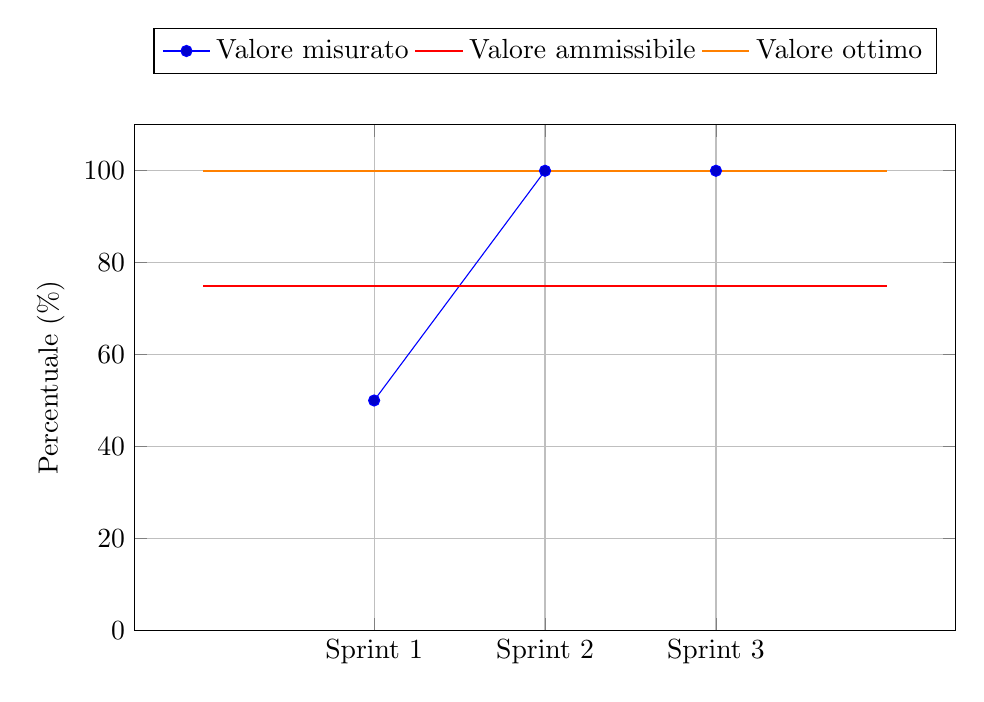
\begin{tikzpicture}
    \begin{axis}[
        width=12cm, height=8cm,
        ymin=0, ymax=110,
        xtick={1, 2, 3},
        xticklabels={Sprint 1, Sprint 2, Sprint 3},
        xlabel={},
        ylabel={Percentuale (\%)},
        grid=major,
        scaled ticks=false,
        legend style={at={(0.5,1.1)}, anchor=south, legend columns=-1},
    ]
    \addplot coordinates {(1, 50) (2, 100) (3, 100)};
    \addlegendentry{Valore misurato}
    \addplot[red, thick] coordinates {(0, 75) (4, 75)};
    \addlegendentry{Valore ammissibile}
    \addplot[orange, thick] coordinates {(0, 100) (4, 100)};
    \addlegendentry{Valore ottimo}
    \end{axis}
\end{tikzpicture}

\subsection*{RTB}

\subsection*{PB}